\documentclass{article}

% if you need to pass options to natbib, use, e.g.:
%     \PassOptionsToPackage{numbers, compress}{natbib}
% before loading neurips_2020

% ready for submission
% \usepackage{neurips_2020}

% to compile a preprint version, e.g., for submission to arXiv, add add the
% [preprint] option:
%     \usepackage[preprint]{neurips_2020}

% to compile a camera-ready version, add the [final] option, e.g.:
%     \usepackage[final]{neurips_2020}

% to avoid loading the natbib package, add option nonatbib:

\usepackage[nonatbib]{neurips_2020}

\usepackage[utf8]{inputenc} % allow utf-8 input
\usepackage[T1]{fontenc}    % use 8-bit T1 fonts
\usepackage{hyperref}       % hyperlinks
\usepackage{url}            % simple URL typesetting
\usepackage{booktabs}       % professional-quality tables
\usepackage{amsfonts}       % blackboard math symbols
\usepackage{nicefrac}       % compact symbols for 1/2, etc.
\usepackage{microtype}      % microtypography

\usepackage{amsfonts}
\usepackage{bm}
\usepackage{tikz}
\usetikzlibrary{bayesnet}
\usetikzlibrary{arrows}
\usepackage{color}
\usepackage{graphicx}
\usepackage{caption}
\usepackage{subcaption}
\usetikzlibrary{backgrounds}
\usepackage{multirow}
\usepackage{algorithm}
\usepackage{algpseudocode}
\usepackage{amsthm}
\usepackage{mathtools}
\usepackage{wrapfig}
\usepackage{txfonts}
\usepackage{stackrel}
\usetikzlibrary{arrows.meta}

\newcommand{\een}{\mathbb{1}}
\newcommand{\vX}{\mathbf{X}}
\newcommand{\vx}{\mathbf{x}}
\newcommand{\vq}{\mathbf{q}}
\newcommand{\vf}{\mathbf{f}}
\newcommand{\ve}{\bm{\epsilon}}
\newcommand{\expectation}{\mathbb{E}}
\newcommand{\contribution}{{\phi}}
\newcommand{\val}{{v}}
\newcommand{\dodo}{\mathit{do}}
\newcommand{\ldo}[1]{\dodo(X_{#1} = x_{#1})}
\newcommand{\lvdo}[1]{\dodo(\vX_{#1} = \vx_{#1})}
\newcommand{\sdo}[1]{\hat{x}_{#1}}
\newcommand{\svdo}[1]{\hat{\vx}_{#1}}
\newcommand{\pa}{\mathop{\textit{pa}}}
\newcommand{\spa}{\mathop{\textit{\scriptsize pa}}}
\newcommand{\perm}{\pi}
\newcommand{\actcont}{\contribution^{\mbox{\scriptsize active}}}
\newcommand{\passcont}{\contribution^{\mbox{\scriptsize passive}}}
\newcommand{\operator}{\mathit{op}}
\newcommand{\sop}[1]{\operator(x_{#1})}
\newcommand{\svop}[1]{\operator(\vx_{#1})}
\newcommand{\lop}[1]{\operator(X_{#1} = x_{#1})}
\newcommand{\lvop}[1]{\operator(\vX_{#1} = \vx_{#1})}
\newcommand{\allfeatures}{{N}}
\newcommand{\bx}{\bar{x}}
\newcommand{\tx}{\tilde{x}}
\newcommand{\hx}{\hat{x}}
\newcommand{\allmeans}{{\cal X}}
\newcommand{\diagbeta}{{\cal B}}
\newcommand{\mapmat}{{\cal M}}
\newcommand{\contmat}{{\cal C}}
\newcommand{\onder}[2]{{#1}_{\mbox{\scriptsize #2}}}
\newcommand{\boven}[2]{#1^{\mbox{\scriptsize #2}}}
\newcommand{\isequal}{\hspace*{-2.5mm} & = & \hspace*{-2.5mm}}
\newcommand{\chaincomponents}{{\cal T}}
\newcommand{\isequaldo}[1]{\hspace*{-2.5mm} & \overset{(#1)}{=} & \hspace*{-2.5mm}}
\newcommand{\Spre}{\underline{S}}
\newcommand{\Spost}{\bar{S}}
\newcommand{\isequaldono}[1]{\overset{(#1)}{=}}

\newcommand{\comment}[1]{{\color{red} #1}}


\newtheorem{theorem}{Theorem}
\newtheorem{corollary}{Corollary}

\title{Supplement of ``Causal Shapley Values: Exploiting Causal Knowledge to Explain Individual Predictions of Complex Models''} 

% The \author macro works with any number of authors. There are two commands
% used to separate the names and addresses of multiple authors: \And and \AND.
%
% Using \And between authors leaves it to LaTeX to determine where to break the
% lines. Using \AND forces a line break at that point. So, if LaTeX puts 3 of 4
% authors names on the first line, and the last on the second line, try using
% \AND instead of \And before the third author name.

%\author{%
%  Pietje Puk\\
%  Radboud University
%  Institute for Computing and Information Sciences\\
%  Nijmegen, The Netherlands \\
%  \texttt{pietje.puk@ru.nl} \\
  % examples of more authors
  % \And
  % Coauthor \\
  % Affiliation \\
  % Address \\
  % \texttt{email} \\
  % \AND
  % Coauthor \\
  % Affiliation \\
  % Address \\
  % \texttt{email} \\
  % \And
  % Coauthor \\
  % Affiliation \\
  % Address \\
  % \texttt{email} \\
  % \And
  % Coauthor \\
  % Affiliation \\
  % Address \\
  % \texttt{email} \\
%}



\begin{document}

\maketitle

\newcommand{\perpsg}{\stackrel[G]{\sigma}{\Perp}}
\newcommand{\vW}{\mathbf{W}}
\newcommand{\vY}{\mathbf{Y}}
\newcommand{\vZ}{\mathbf{Z}}

\section{\textit{Do}-calculus for cyclic graphs}

For completeness, we here repeat the rules of {\em do}-calculus for cyclic graphs, in the notation of~\cite{forre2019causal}, which generalizes~\cite{pearl2012calculus}. We are given a causal graph $G$. To each node $X_i$ which is intervened upon, we add an `intervention node' $I_{X_i}$, with a directed edge from $I_{X_i}$ to $X_i$ that we clamp to the value $x_i$. The corresponding graph is called $\hat{G}^+$. $\hat{G}_{\dodo(\vW)}$ is now obtained by removing from $\hat{G}^+$ all incoming edges to variables that are part of $\vW$, except those from the corresponding intervention nodes $I_{\vW}$. We use shorthand
\[
\vY \perpsg \vX ~|~ \vZ, \dodo(\mathbf{W})
\]
to indicate that $\vY$ and $\vX$ are $\sigma$-separated by $\vZ$ in the graph $\hat{G}_{\dodo(\vW)}$.  $\sigma$-separation is a generalization of standard d-separation (see~\cite{forre2019causal} for details).

\textit{Do}-calculus now consists of the following three inference rules that can be used to map interventional and observational distributions.
\begin{enumerate}
	\item Insertion/deletion of observation:
	\[
	 P(\vY|\vX,\vZ,\dodo(\vW)) = P(\vY|\vZ,\dodo(\vW)) \mbox{~~if~~} \vY \perpsg \vX ~|~ \vZ,\dodo(\vW) \: .
	\]
	\item Action/observation exchange:
	\[
	P(\vY|\dodo(\vX),\vZ,\dodo(\vW)) = P(\vY|\vX,\vZ,\dodo(\vW)) \mbox{~~if~~} \vY \perpsg I_{\vX} ~|~ \vX, \vZ, \dodo(\vW)  \: .
	\]
	\item Insertion/deletion of actions:
	\[
	P(\vY|\dodo(\vX),\vZ,\dodo(\vW)) = P(\vY|\vZ,\dodo(\vW)) \mbox{~~if~~} \vY \perpsg I_{\vX} ~|~ \vZ,\dodo(\vW) \: .
	\]	
\end{enumerate}
Through consecutive application of these rules, we can try to turn any interventional probability of interest into an observational probability.

\section{Shapley values for linear models}

\begin{figure}
		\centering
		\tikzstyle{arrow} = [thick,->,>=stealth]
		\tikzstyle{dashedarrow} = [thick,->,>=stealth,dashed]
		\tikz{
			% causal chain
			\node[latent] at (0,0) (y1) {$Y$};%
			\node[latent] at (0,1.5) (x12) {$X_2$};
			\node[latent] at (0,3) (x11) {$X_1$};
			\node[text height=1em, anchor=north] at (0,4.2) {Chain and fork};
			\draw[arrow] (x12) -- node[anchor=west]{$\beta_2$} (y1);
			\draw[arrow] (x11) -- (x12);
			\draw[arrow] (x11) to[bend right] node[anchor=east]{$\beta_1$}(y1);
			% common confounder
			\node[latent] at (3,0) (y3) {$Y$};
			\node[latent] at (3,1.5) (x32) {$X_2$};
			\node[latent] at (3,3) (x31) {$X_1$};
			\node[latent] at (3.6,2.25) (z)  {$Z$};
			\node[text height=1em, anchor=north] at (3,4.2) {Confounder};
			\draw[arrow] (x32) -- node[anchor=west]{$\beta_2$} (y3);
			\draw[arrow] (z) -- (x31);
			\draw[arrow] (z) -- (x32);
			\draw[arrow] (x31) to[bend right] node[anchor=east]{$\beta_1$}(y3);
			% cycle
			\node[latent] at (6,0) (y4) {$Y$};%
			\node[latent] at (6,1.5) (x42) {$X_2$};
			\node[latent] at (6,3) (x41) {$X_1$};
			\node[text height=1em, anchor=north] at (6,4.2) {Cycle};
			\draw[arrow] (x42) -- node[anchor=west]{$\beta_2$} (y4);
			\draw[arrow] (x41) to[bend left=15] (x42);
			\draw[arrow] (x42) to[bend left=15] (x41);
			\draw[arrow] (x41) to[bend right] node[anchor=east]{$\beta_1$}(y4);			
		}
	\caption{Three causal models with the same observational distribution over features, yet a different causal structure. To connect to the models in the main text, we set $\beta_1 = 0$ and $\beta_2 = \beta$, except that for the `fork' we set $\beta_2 = 0$, $\beta_1 = \beta$, and then swap the indices.}
	\label{fig:threemodels}
\end{figure}

We will make use of the {\em do}-calculus rules above to derive the causal Shapley values for the four different models in Figure~1 in the main text. To this end, we consider the three models in Figure~\ref{fig:threemodels} that predict $f(x_1,x_2) = \beta_1 x_1 + \beta_2 x_2$ for general values of $\beta_1$ and $\beta_2$. All three models have the same observational probability distribution, with $\expectation[X_i] = \bx_i$ and $\expectation[X_{3-i}] = \alpha_i x_i$, for $i = 1,2$, yet different causal structures. We will arrive at the main text's results for the `chain', `confounder', and `cycle' by setting $\beta_1 = 0$, whereas for the `fork' we set $\beta_2 = 0$ and swap the two indices. We then further need to take $\bx_1 = \bx_2 = 0$, and $\alpha = \alpha_2$.

Following the definitions in the main text, the contribution of feature $i$ given permutation $\perm$ is the difference in value function before and after setting the feature to its value:
\begin{equation}
\contribution_i(\perm) = \val(\{j: j \preceq_\perm i\}) - \val(\{j: j \prec_\perm i\}) \: ,
\label{eq:contperm}
\end{equation}
with value function
\begin{equation}
\val(S) = \expectation \left[f(\vX) | \lvdo{S} \right] = \int d\vX_{\bar{S}} \: P(\vX_{\bar{S}}|\svdo{S}) f(\vX_{\bar{S}},\vx_S) \: ,
\label{eq:valuedef}
\end{equation}
where we use shorthand $\svdo{}$ for $\lvdo{}$. Combining these two definitions and substituting $f(\vx) = \sum_i \beta_i x_i$, we obtain
\[
\contribution_i(\perm) =
\beta_i \left(x_i - \expectation [X_i | \svdo{j: j \prec_\perm i}]\right) + \sum_{k \succ_\perm i} \beta_k \left( \expectation [X_k | \svdo{j: j \preceq_\perm i}] - \expectation [X_k | \svdo{j: j \prec_\perm i}] \right) \: .
\]
The first term corresponds to the direct effect, the second one to the indirect effect. Symmetric causal Shapley values will follow by averaging these contributions for the two possible permutations $\perm = (1,2)$ and $\perm = (2,1)$. Conditional Shapley values result when replacing conditioning by intervention with conventional conditioning by observation, marginal Shapley values by not conditioning at all.

To start with the latter, we immediately see that for {\em marginal Shapley values} the indirect effect vanishes and the direct effect simplifies to
\[
\phi_i = \phi_i(\perm) = \beta_i (x_i - \expectation[X_i])  = \beta_i (x_i - \bx_i) \: ,
\]
as also derived in~\cite{aas2019explaining}.

For symmetric conditional Shapley values, we do get different contributions for the two different permutations, but by definition still the same for the three different models:
\begin{eqnarray}
\phi_1(1,2) \isequal \beta_1 (x_1 - \expectation[X_1]) + \beta_2 (\expectation[X_2|x_1] - \expectation[X_2]) = \beta_1 (x_1 - \bx_1) + \beta_2 \alpha_1 (x_1 - \bx_1) \nonumber \\
\phi_2(1,2) \isequal \beta_2 (x_2 - \expectation[X_2|x_1]) = \beta_2 (x_2 - \bx_2) - \beta_2 \alpha_1 (x_1 - \bx_1) \: .
\label{eq:asymmetric}
\end{eqnarray}
Here the first term in the contribution for the first feature corresponds to the direct effect and the second term to the indirect effect. The contribution for the second feature only consists of a direct effect. The contributions for the other permutation follow by swapping the indices and the final Shapley values by averaging to arrive at the {\em symmetric conditional Shapley values}
\begin{eqnarray}
\phi_1 \isequal \beta_1 (x_1 - \bx_1) - {1 \over 2} \beta_1 \alpha_2 (x_2 - \bx_2) + {1 \over 2} \beta_2 \alpha_1 (x_1 - \bx_1) \nonumber \\
\phi_2 \isequal \beta_2 (x_2 - \bx_2) - {1 \over 2} \beta_2 \alpha_1 (x_1 - \bx_1) + {1 \over 2} \beta_1 \alpha_2 (x_2 - \bx_2) \: ,
\label{eq:symmetric}
\end{eqnarray}
where now the first two terms constitute the direct effect and the third term the indirect effect.

\begin{table}
\begin{center}
\begin{tabular}{r|ccc} \toprule
expectation & chain & confounder & cycle \\ \midrule
$\expectation[X_1|\sdo{2}]$ & $\expectation[X_1]$ & $\expectation[X_1]$ & $\expectation[X_1|x_2]$ \\
$\expectation[X_2|\sdo{1}]$ & $\expectation[X_2|x_1]$ & $\expectation[X_2]$ & $\expectation[X_2|x_1]$ \\
\bottomrule
\end{tabular}
\end{center}
\caption{Turning expectations under conditioning by intervention into expectations under conventional conditioning by observation for the three models in Figure~\ref{fig:threemodels}.}
\label{tab:rewriting}
\end{table}

The {\em asymmetric conditional Shapley values} consider both permutations for the confounder and the cycle, and hence are equivalent to the symmetric Shapley values for those models. Yet for the chain, they only consider the permutation $\perm(1,2)$ and thus yield $\bm{\phi} = \bm{\phi}(1,2)$ from~(\ref{eq:asymmetric}).

To go from the symmetric conditional Shapley values to the causal symmetric Shapley values, we follow the same line of reasoning, but have to replace $\expectation[X_2|x_1]$ by $\expectation[X_2|\sdo{1}]$ and $\expectation[X_1|x_2]$ by $\expectation[X_1|\sdo{2}]$. Table~\ref{tab:rewriting} tells whether
the expectations under conditioning by intervention reduce to expectations under conditioning by observation (because of the second rule of \textit{do}-calculus above) or to marginal expectations (because of the third rule). For the chain we have
\[
P(X_2 | \sdo{1}) = P(X_2 | x_1) \mbox{~~since~~} X_2 \perpsg I_{X_1} ~|~ X_1 \mbox{~~(rule 2),~yet~~} P(X_1 | \sdo{2}) = P(X_1) \mbox{~~since~~} X_1 \perpsg I_{X_2} \mbox{~~(rule 3),}
\]
for the confounder
\[
P(X_2 | \sdo{1}) = P(X_2) \mbox{~~since~~} X_2 \perpsg I_{X_1}  \mbox{~~and~~} P(X_1 | \sdo{2}) = P(X_1) \mbox{~~since~~} X_1 \perpsg I_{X_2} \mbox{~~(rule 3),}
\]
and for the cycle
\[
P(X_2 | \sdo{1}) = P(X_2 | x_1) \mbox{~~since~~} X_2 \perpsg I_{X_1} ~|~ X_1 \mbox{~~and~~} P(X_1 | \sdo{2}) = P(X_1|x_2) \mbox{~~since~~} X_1 \perpsg I_{X_2} ~|~ X_2 \mbox{~~(rule 2).}
\]
Consequently, for the confounder the {\em symmetric} and {\em asymmetric causal Shapley values} coincide with the marginal Shapley values (consistent with~\cite{janzing2019feature}) and for the cycle with the symmetric conditional Shapley values from~(\ref{eq:symmetric}). For the chain, the causal symmetric Shapley values become
\begin{eqnarray}
\phi_1(1,2) \isequal \beta_1 (x_1 - \bx_1) + {1 \over 2} \beta_2 \alpha_1 (x_1 - \bx_1) \nonumber \\
\phi_2(1,2) \isequal \beta_2 (x_2 -\bx_2) - {1 \over 2} \beta_2 \alpha_1 (x_1 - \bx_1) \: ,
\label{eq:asymmetric}
\end{eqnarray}
where the asymmetric causal Shapley values coincides with the asymmetric conditional Shapley values from~(\ref{eq:asymmetric}).

Collecting all results and setting $\bx_1 = \bx_2 = \beta_1 = 0$, $\beta_2 = \beta$, and $\alpha_1 = \alpha$ (after swapping the indices for the `fork'), we arrive at the Shapley values reported in Figure~1 in the main text. Note that for most Shapley values, the indirect effect for the second feature vanishes because we chose to set $\beta_1 = 0$. The exceptions, apart from the marginal Shapley values, are the causal Shapley values for the chain and the confounder, as well as the asymmetric conditional Shapley values for the chain: these show no indirect effect for the second feature even for nonzero $\beta_1$.

\section{Proofs and corollaries on causal chain graphs}

In this section we expand on the proof of Theorem~1 in the main text and add some corollaries to link back to other approaches for computing Shapley values.

The probability distribution for a causal chain graph reads
\begin{equation}
P(\vX) = \prod_{\tau \in \chaincomponents} P(\vX_\tau|\vX_{\spa(\tau)}) \: .
\label{eq:chaingraph}
\end{equation}
For each chain component, we further need to specify whether  (surplus) dependencies within the component are due to confounding or due to mutual interactions. Given this information, we can turn any causal query into an observational distribution with the following interventional formula.

\begin{theorem}
	For causal chain graphs, we have the interventional formula 
	\begin{eqnarray}
	P(\vX_{\bar{S}}|\lvdo{S}) \isequal \prod_{\tau \in \chaincomponents_{\textrm{\upshape \scriptsize confounding}}} P(\vX_{\tau \cap \bar{S}}|\vX_{\spa(\tau)  \cap \bar{S}},\vx_{\spa(\tau) \cap S}) \times \nonumber \\
	&& \prod_{\tau \in \chaincomponents_{\overline{\textrm{\upshape \scriptsize confounding}}}} P(\vX_{\tau \cap \bar{S}}|\vX_{\spa(\tau) \cap \bar{S}},\vx_{\spa(\tau) \cap S},\vx_{\tau \cap S}) \: .
	\label{eq:chaininterventional}
	\end{eqnarray}
\end{theorem}

\begin{proof}
Plugging in~(\ref{eq:chaingraph}) and using shorthand $\svdo{} = \lvdo{}$, we obtain
\[
P(\vX_{\bar{S}}|\svdo{S}) = P(\vX|\svdo{S})
\isequaldono{1} \prod_{\tau \in \chaincomponents} P(\vX_\tau|\vX_{\spa(\tau)},\svdo{S}) = \prod_{\tau \in \chaincomponents} P(\vX_{\tau \cap \bar{S}}|\vX_{\spa(\tau)  \cap \bar{S}},\svdo{S})
\]
where in the second step we implicitly made use of {\em do}-calculus rule~(1): the conditional independencies in the causal chain graph are preserved when we intervene on some of the variables.

Now rule~(3) tells us that we can ignore any interventions from nodes in components further down the causal chain graph as well as those from higher up that are shielded by the direct parents:
\[
P(\vX_{\tau \cap \bar{S}}|\vX_{\spa(\tau)  \cap \bar{S}},\svdo{S})
\isequaldono{3} P(\vX_{\tau \cap \bar{S}}|\vX_{\spa(\tau)  \cap \bar{S}},\svdo{\spa(\tau) \cap S},\svdo{\tau \cap S}) \: .
\]
Rule~(2) then states that conditioning by intervention upon variables higher up in the causal chain graph is equivalent to conditioning by observation:
\[
P(\vX_{\tau \cap \bar{S}}|\vX_{\spa(\tau)  \cap \bar{S}},\svdo{\spa(\tau) \cap S},\svdo{\tau \cap S}) \isequaldono{2}
P(\vX_{\tau \cap \bar{S}}|\vX_{\spa(\tau)  \cap \bar{S}},\vx_{\spa(\tau) \cap S},\svdo{\tau \cap S}) \: .
\]
For a chain component with dependencies induced by a common confounder, rule (3) applies once more and makes that we can ignore the interventions:
\[
P(\vX_{\tau \cap \bar{S}}|\vX_{\spa(\tau)  \cap \bar{S}},\vx_{\spa(\tau) \cap S},\svdo{\tau \cap S}) = P(\vX_{\tau \cap \bar{S}}|\vX_{\spa(\tau)  \cap \bar{S}},\vx_{\spa(\tau) \cap S}) \: .
\]
For a chain component with dependencies induced by mutual interactions, rule (2) again applies and allows us to replace conditioning by intervention with conditioning by observation:
\[
P(\vX_{\tau \cap \bar{S}}|\vX_{\spa(\tau)  \cap \bar{S}},\vx_{\spa(\tau) \cap S},\svdo{\tau \cap S}) = P(\vX_{\tau \cap \bar{S}}|\vX_{\spa(\tau)  \cap \bar{S}},\vx_{ \spa(\tau) \cap S},\vx_{\tau \cap S})) \: .
\]
\end{proof}

Algorithm~\ref{alg:sampling} provides pseudocode on how to estimate the value function $\val(S)$ by drawing samples from the interventional probability~(\ref{eq:chaininterventional}). It assumes that a user has specified a partial causal ordering of the features, which is translated to a chain graph with components $\chaincomponents$, and for each (non-singleton) component $\tau$ whether or not surplus dependencies are the result of confounding. Other prerequisites include access to the model $f()$, the feature vector $\vx$, (a procedure to sample from) the observational probability distribution $P(\vX)$, and the number of samples $\onder{N}{samples}$.

\begin{algorithm}[t]
	\caption{Compute the value function $\val(S)$ under conditioning by intervention.}
	\label{alg:sampling}
	\begin{algorithmic}[1]
		\Function{ValueFunction}{$S$}
		\For{$k \gets 1 \mbox{~to~} \onder{N}{samples}$}
		\ForAll{$j \gets 1 \mbox{~to~} |\chaincomponents|$} \Comment{run over all chain components in their causal order}
			\If{confounding$(\tau_j)$} 
				\ForAll{$i \in \tau_j \cap \bar{S}$}
					\State Sample $\tilde{x}_i^{(k)} \sim P(X_i|\tilde{\vx}_{\spa(\tau_j) \cap \bar{S}}^{(k)},\vx_{\spa(\tau_j) \cap \bar{S}})$ \Comment{can be drawn independently}
				\EndFor
			\Else
				\State Sample $\tilde{\vx}_{\tau_j \cap \bar{S}}^{(k)} \sim P(\vX_{\tau_j \cap \bar{S}}|\tilde{\vx}_{\spa(\tau_j) \cap \bar{S}}^{(k)},\vx_{\spa(\tau_j) \cap \bar{S}},\vx_{\tau_j \cap S})$ \Comment{e.g., Gibbs sampling}
			\EndIf
		\EndFor
		\EndFor
		\State $\val \gets {\displaystyle {1 \over \onder{N}{samples}} \sum_{k=1}^{\onder{N}{samples}} f(\vx_S,\tilde{\vx}_{\bar{S}}^{(k)})}$
		\State \Return $\val$
		\EndFunction
	\end{algorithmic}
\end{algorithm}

Theorem~1 connects to observations made and algorithms proposed in recent papers.
\begin{corollary}
	With all features combined in a single component and all dependencies induced by confounding, as in~\cite{janzing2019feature}, causal Shapley values are equivalent to marginal Shapley values. 
\end{corollary}
\begin{proof}
	{\em Do}-calculus rule~(3) yields $P(\vX_{\bar{S}}|\svdo{S}) = P(\vX_{\bar{S}})$ for all subsets $S$, i.e., as if all features are independent.
\end{proof}
\begin{corollary}
	With all features combined in a single component and all dependencies induced by mutual interactions, causal Shapley values are equivalent to conditional Shapley values as proposed in~\cite{aas2019explaining}.
\end{corollary}
\begin{proof}
	Now, {\em do}-calculus rule~(2) applies and gives $P(\vX_{\bar{S}}|\svdo{S}) = P(\vX_{\bar{S}}|\vx_{S})$ for all subsets $S$, which boils down to conventional conditioning by observation.
\end{proof}
\begin{corollary}
	When we only take into account permutations that match the causal ordering and assume that all dependencies within chain components are induced by mutual interactions, the resulting asymmetric causal Shapley values are equivalent to the asymmetric conditional Shapley values as defined in~\cite{frye2019asymmetric}.
\end{corollary}
\begin{proof}
	Following~\cite{frye2019asymmetric}, asymmetric Shapley values only include those permutations $\perm$ for which $i \prec_\perm j$ for all known ancestors $i$ of descendants $j$ in the causal graph. For those permutations, we are guaranteed to have $\tau \prec_G \tau'$ for all $\tau, \tau' \in \mathcal{T}$ such that $\tau \cap S \neq \emptyset, \tau' \cap \bar{S} \neq \emptyset$. That is, the chain components that contain features from $S$ are never later in the causal ordering of the chain graph $G$ than those that contain features from $\bar{S}$. We then have
	\[
	P(\vX_{\bar{S}}|\vx_S) = \prod_{\tau \in \chaincomponents} P(\vX_{\tau \cap \bar{S}}|\vX_{\spa(\tau)  \cap \bar{S}},\vx_{S}) = \prod_{\tau \in \chaincomponents} P(\vX_{\tau \cap \bar{S}}|\vX_{\spa(\tau)  \cap \bar{S}},\vx_{\spa(\tau) \cap S},\vx_{\tau \cap S}) = P(\vX_{\bar{S}}|\svdo{S}) \: ,
	\]
	where in the last step we used interventional formula~(\ref{eq:chaininterventional}) in combination with the fact that $\onder{\chaincomponents}{confounding} = \emptyset$.
\end{proof}

\section{Additional illustrations on the bike rental data}

Figure~\ref{fig:sinaplots} shows sina plots for asymmetric conditional Shapley values (left) and marginal Shapley values (right), to be compared with the sina plots for symmetric causal Shapley values in Figure~3 of the main text. The sina plots for asymmetric causal Shapley values are virtually indistinguishable from those for the asymmetric conditional Shapley values.

It can be seen that the marginal Shapley values strongly focus on temperature, largely ignoring the seasonal variables. The asymmetric Shapley values do the opposite: they focus on the seasonal variables, in particular {\em cosyear} and put much less emphasis on the temperature variables.

\begin{figure}[t]
	\centering
	\begin{minipage}{.49\linewidth}
%		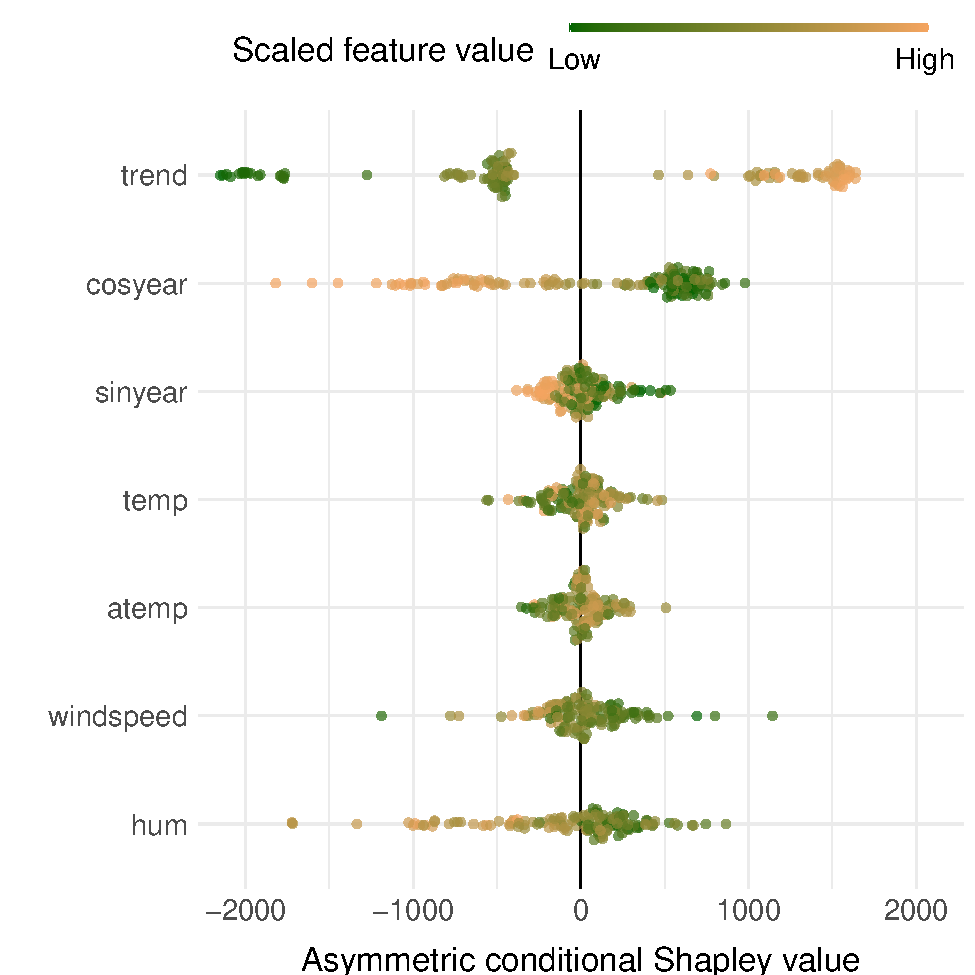
\includegraphics[width=\textwidth]{figures/sina_plot_asymmetric.pdf}
	\end{minipage}
	\begin{minipage}{.49\linewidth}
%		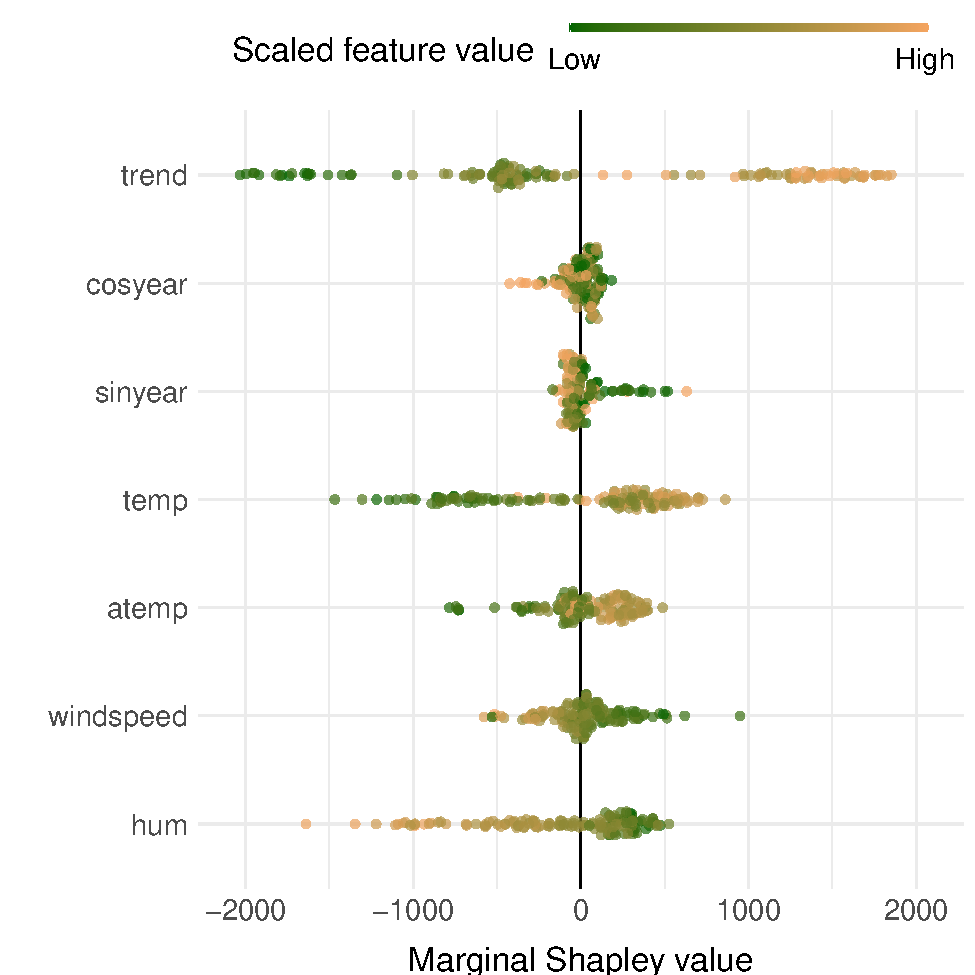
\includegraphics[width=\textwidth]{figures/sina_plot_marginal.pdf}
	\end{minipage}
	\caption{Sina plots of asymmetric (conditional) Shapley values (left) and marginal Shapley values (right). See Figure~3 in the main text for further details.}
	\label{fig:sinaplots}
\end{figure}

\bibliography{shapleyrefs}
\bibliographystyle{plain}


\end{document}
